\chapter*{ANEXO A: Resultados extendidos}
\label{ch:anexo}

En este capítulo se muestra el detalle numérico de las métricas componentes de $CMOPSO-CLAHE$, además de valores resultantes de las variables de decisión y tiempos de ejecución para las imágenes de prueba, para los resultados no dominados. Los tiempos de ejecución detallados corresponden a \texttt{time())} \cite{time}.

%Los resultados de este apartado son los promedios de los tiempos de ejecución, de los algoritmos \textit{Histogram Equalization} (HE), \textit{Multiscale Morphological Contrast Enhancement} (MMCE) y el algoritmo propuesto, para las 200 imágenes en escala de grises. Los algoritmos se implementaron con el framewok ImageJ y se hizo ejecutar 5 veces los experimentos. En la Tabla \ref{tabla22} se muestran los promedios de los tiempos de ejecución del algoritmo HE para las imágenes en escala de grises.

\scriptsize
\begin{longtable}{|c|c|c|c|c|c|c|c|}
% \centering
%\begin{tabular}
\hline
ID & $\mathscr{R}_x$ & $\mathscr{R}_y$ & $\mathscr{C}$ & $f_1(I,\vv{x})$ & $f_2(I,\vv{x})$ & $f_3(I,\vv{x})$ & $f_4(I,\vv{x})$ \\
0 & 23.6165403175 & 2.69540303852 & 0.0 & 0.0292377 & 0.425724 & 0.412724 & 0.426577 \\
1 & 20.8806065105 & 2.83866806018 & 0.0 & 0.030087 & 0.42386 & 0.410826 & 0.424771 \\
2 & 17.1618809206 & 2.65596140692 & 0.0 & 0.0318866 & 0.421223 & 0.40784 & 0.422096 \\
3 & 14.6055937685 & 3.24210935022 & 0.0 & 0.0322351 & 0.418567 & 0.405405 & 0.419644 \\
4 & 16.3175125499 & 2.65246124014 & 0.0 & 0.0325675 & 0.418894 & 0.405988 & 0.420157 \\
5 & 11.7648539964 & 2.85584979467 & 0.0 & 0.0340767 & 0.413031 & 0.399763 & 0.414117 \\
6 & 7.9831044542 & 2.54774686553 & 0.0 & 0.0365424 & 0.401675 & 0.388628 & 0.402692 \\
7 & 18.0967037678 & 2.0 & 0.0 & 0.038238 & 0.41038 & 0.396594 & 0.414668 \\
8 & 9.50558744928 & 2.81072780661 & 0.0 & 0.0391212 & 0.410855 & 0.397602 & 0.411904 \\
9 & 13.8286043587 & 2.0 & 0.0 & 0.0397372 & 0.406896 & 0.392824 & 0.411252 \\
10 & 9.17661450659 & 3.03582192974 & 0.0 & 0.0419288 & 0.406245 & 0.393219 & 0.407594 \\
11 & 9.37091048983 & 2.0 & 0.0 & 0.0425715 & 0.394656 & 0.380667 & 0.39842 \\
12 & 7.7880055187 & 2.0 & 0.0 & 0.0488863 & 0.389568 & 0.375398 & 0.392996 \\
13 & 6.76474913481 & 2.0 & 0.0 & 0.0519342 & 0.389407 & 0.374979 & 0.392855 \\
14 & 5.05067508004 & 2.9107025755 & 0.0 & 0.0532846 & 0.383024 & 0.369461 & 0.383779 \\
15 & 5.7406442902 & 2.0 & 0.0 & 0.0570464 & 0.38065 & 0.366103 & 0.383668 \\
16 & 4.59028307145 & 2.0 & 0.0 & 0.0581956 & 0.370847 & 0.355854 & 0.372697 \\
17 & 2.0 & 4.95813861442 & 0.0 & 0.0678334 & 0.332408 & 0.319416 & 0.329963 \\
18 & 2.0 & 3.66304838881 & 0.0 & 0.083076 & 0.330307 & 0.315432 & 0.327533 \\
19 & 2.35492574942 & 3.39983773851 & 0.0 & 0.107766 & 0.300927 & 0.288565 & 0.302558 \\
20 & 2.0 & 2.0 & 0.0 & 0.130446 & 0.288674 & 0.274897 & 0.29182 \\
21 & 37.1680210937 & 4.02913470221 & 0.421103062234 & 0.388474 & 0.0796014 & 0.0715557 & 0.0737911 \\
22 & 44.2744458915 & 3.06660345481 & 0.177772531513 & 0.420316 & 0.0571285 & 0.0508797 & 0.0542069 \\
23 & 2.0 & 2.78790539363 & 1.0 & 0.422673 & 0.0391384 & 0.0356485 & 0.0375976 \\
24 & 2.0261623037 & 2.63491553158 & 0.966457510597 & 0.441196 & 0.0358967 & 0.0326292 & 0.0344847 \\
25 & 2.0 & 2.89515796966 & 0.909807336447 & 0.452317 & 0.0334806 & 0.0305298 & 0.0321478 \\
26 & 2.02503785011 & 3.30462032726 & 0.871347872644 & 0.460282 & 0.0313939 & 0.0285593 & 0.0301892 \\
27 & 2.02513727851 & 3.30980113609 & 0.838052371298 & 0.472741 & 0.0288693 & 0.0262626 & 0.0277464 \\
28 & 2.0 & 3.49518428712 & 0.78970323092 & 0.483203 & 0.0264133 & 0.0241076 & 0.0254163 \\
29 & 2.24237960592 & 3.14985091448 & 0.763073541042 & 0.494502 & 0.0247892 & 0.0225578 & 0.0238702 \\
30 & 2.0 & 3.36431215991 & 0.734387233109 & 0.505156 & 0.0216592 & 0.0196863 & 0.0208914 \\
31 & 2.20979700028 & 2.75516146016 & 0.689415824019 & 0.516532 & 0.0201843 & 0.0183705 & 0.0194163 \\
32 & 2.0 & 2.63617326662 & 0.674049273864 & 0.530366 & 0.0177617 & 0.0161534 & 0.0170947 \\
33 & 2.00636569548 & 2.81293702399 & 0.620573402397 & 0.544854 & 0.0155038 & 0.0140995 & 0.0149364 \\
34 & 2.0219725871 & 2.79503388526 & 0.594946439658 & 0.567288 & 0.0141571 & 0.0127951 & 0.0135701 \\
35 & 2.00078360943 & 3.17871015507 & 0.525728438652 & 0.571877 & 0.0115625 & 0.0105159 & 0.011121 \\
36 & 2.00195241245 & 2.94859488298 & 0.5 & 0.588363 & 0.0108908 & 0.00987159 & 0.0104669 \\
37 & 2.0 & 3.0678111982 & 0.483071040731 & 0.59779 & 0.00906811 & 0.00822819 & 0.00867055 \\
38 & 2.0 & 5.82595208171 & 0.456916541899 & 0.611275 & 0.00897331 & 0.00823064 & 0.00851013 \\
39 & 2.26459968878 & 2.78708768442 & 0.428434700311 & 0.614437 & 0.00742514 & 0.00670994 & 0.00714773 \\
40 & 2.00104865637 & 3.22597690322 & 0.390144531289 & 0.628389 & 0.00650833 & 0.00588966 & 0.00621115 \\
41 & 2.00248130651 & 4.35167770908 & 0.38446541693 & 0.631133 & 0.00581047 & 0.00528148 & 0.00556787 \\
42 & 2.0 & 3.35300114946 & 0.37527195105 & 0.64904 & 0.0048614 & 0.00438096 & 0.00457561 \\
43 & 2.0 & 3.68515652281 & 0.31193055736 & 0.65892 & 0.00444588 & 0.0039587 & 0.00415919 \\
44 & 2.0 & 3.37001662175 & 0.310920748974 & 0.667173 & 0.00401135 & 0.00358585 & 0.00381668 \\
45 & 2.0 & 4.24860032483 & 0.290295960924 & 0.681955 & 0.00282212 & 0.002562 & 0.002621 \\
46 & 2.0 & 3.00776846152 & 0.244028880272 & 0.698645 & 0.00224598 & 0.00200366 & 0.00205784 \\
47 & 2.42511211594 & 3.29117230901 & 0.198283113397 & 0.708029 & 0.00164594 & 0.0014135 & 0.00148235 \\
48 & 2.0 & 3.28183678382 & 0.150847773862 & 0.721569 & 0.00132173 & 0.00109436 & 0.00111522 \\
49 & 2.20521157676 & 5.56409489743 & 0.161790895768 & 0.744286 & 0.00127126 & 0.00105903 & 0.00109671 \\
50 & 2.00464193873 & 2.47291746645 & 0.153546446329 & 0.744481 & 0.00108487 & 0.000878814 & 0.000907648 \\
51 & 3.40819206284 & 3.29931389251 & 0.145704588048 & 0.747523 & 0.00103455 & 0.000816322 & 0.000848165 \\
52 & 2.0 & 3.62408439102 & 0.146162992336 & 0.753901 & 0.000827484 & 0.000614913 & 0.000645663 \\
53 & 2.22704667142 & 2.0 & 0.112761751028 & 0.759912 & 0.000615229 & 0.00043859 & 0.000453515 \\
54 & 2.00188488663 & 3.47606755787 & 0.00011646417386 & 0.775049 & 0.000299272 & 0.000143607 & 0.000141378 \\
55 & 2.81673525126 & 2.9239906217 & 0.00178837395609 & 0.786418 & 0.000323289 & 0.000143135 & 0.000182232 \\
56 & 2.0 & 2.0 & 0.0281221731315 & 0.788927 & 0.000204143 & 5.26475e-05 & 5.18143e-05 \\
 \hline
\multicolumn{8}{|c|}{\textbf{Tiempos de ejecución:} \texttt{real:70m10.567s,user:207m55.583s,sys:95m37.939s}}\\  \hline
% \end{tabular}
\caption{Resultados no dominados para la imagen de prueba \texttt{calhouse\_230.jpg}}
\label{tab:calhouse_230}
\end{longtable}
\normalsize

\begin{figure}[H]
    \centering
    %\begin{subfigure}[t]{0.45\textwidth}
    \begin{subfigure}[ID=0]{
        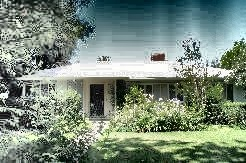
\includegraphics[width=0.45\textwidth]{./Figures/calhouse_230/0-resultado.jpg}
    }
%        \caption{Imagen Original. $\mathscr{H_Y}=0.207231$, $SSIM_R=1$, $SSIM_G=1$, $SSIM_B=1$}
        \label{fig:calhouse2300}
    \end{subfigure}
    ~ %add desired spacing between images, e. g. ~, \quad, \qquad, \hfill etc. 
      %(or a blank line to force the subfigure onto a new line)
    \begin{subfigure}[DI=1]{
        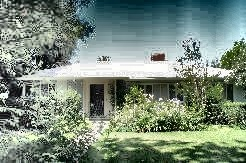
\includegraphics[width=0.45\textwidth]{./Figures/calhouse_230/1-resultado.jpg}   
    }
    %\begin{subfigure}[t]{0.45\textwidth}
%        \caption{Enhanced Image. $\mathscr{H_Y}=0.611275$, $SSIM_R=0.00897331$, $SSIM_G=0.00823064$, $SSIM_B=0.00851013$}
        \label{fig:calhouse2301}
    \end{subfigure}
    ~ %add desired spacing between images, e. g. ~, \quad, \qquad, \hfill etc. 
    %(or a blank line to force the subfigure onto a new line)
    \begin{subfigure}[ID=23]{
        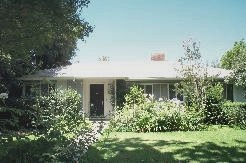
\includegraphics[width=0.45\textwidth]{./Figures/calhouse_230/23-resultado.jpg}
    }
    % \begin{subfigure}[t]{0.45\textwidth}
%        \caption{Enhanced Image.  $\mathscr{H_Y}=0.0350595$, $SSIM_R=0.416776$, $SSIM_G=0.403636$, $SSIM_B=0.417654$}
        \label{fig:calhouse23023}
    \end{subfigure} 
    \begin{subfigure}[ID=24]{
        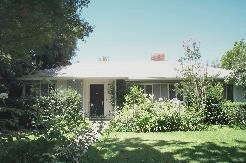
\includegraphics[width=0.45\textwidth]{./Figures/calhouse_230/24-resultado.jpg}
    }
    % \begin{subfigure}[t]{0.45\textwidth}
        %\caption{Enhanced Image using \cite{morepso}. $\mathscr{H_Y}=0.788927$, $SSIM_R=0.000204143$, $SSIM_G=0.0000526475$, $SSIM_B=0.0000518143$}
        \label{fig:calhouse23024}
    \end{subfigure}
    ~ %add desired spacing between images, e. g. ~, \quad, \qquad, \hfill etc. 
    %(or a blank line to force the subfigure onto a new line)
    \begin{subfigure}[ID=56]{
        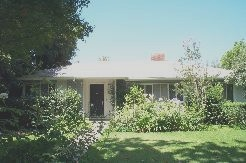
\includegraphics[width=0.45\textwidth]{./Figures/calhouse_230/56-resultado.jpg}
    }
    % \begin{subfigure}[t]{0.45\textwidth}
%        \caption{Enhanced Image.  $\mathscr{H_Y}=0.0350595$, $SSIM_R=0.416776$, $SSIM_G=0.403636$, $SSIM_B=0.417654$}
        \label{fig:calhouse23056}
    \end{subfigure} 
    \begin{subfigure}[Imagen Original]{
        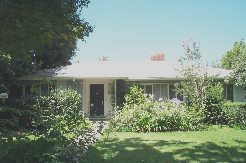
\includegraphics[width=0.45\textwidth]{./Figures/calhouse_230/calhouse_230.jpg}
    }
    % \begin{subfigure}[t]{0.45\textwidth}
        %\caption{Enhanced Image using \cite{morepso}. $\mathscr{H_Y}=0.788927$, $SSIM_R=0.000204143$, $SSIM_G=0.0000526475$, $SSIM_B=0.0000518143$}
        \label{fig:calhouse230orig}
    \end{subfigure}
    \caption{Imágenes visualmente relevantes obtenidas mediante $CMOPSO-CLAHE$. Las variables y decisión y métricas de las imágenes se muestran en la tabla \ref{tab:calhouse_230}.}\label{fig:anexocalhouse230}
\end{figure}

\scriptsize
\begin{longtable}{|c|c|c|c|c|c|c|c|}
% \centering
%\begin{tabular}
\hline
ID & $\mathscr{R}_x$ & $\mathscr{R}_y$ & $\mathscr{C}$ & $f_1(I,\vv{x})$ & $f_2(I,\vv{x})$ & $f_3(I,\vv{x})$ & $f_4(I,\vv{x})$ \\
0 & 23.6165403175 & 2.69540303852 & 0.0 & 0.0292377 & 0.425724 & 0.412724 & 0.426577 \\
1 & 20.8806065105 & 2.83866806018 & 0.0 & 0.030087 & 0.42386 & 0.410826 & 0.424771 \\
2 & 17.1618809206 & 2.65596140692 & 0.0 & 0.0318866 & 0.421223 & 0.40784 & 0.422096 \\
3 & 14.6055937685 & 3.24210935022 & 0.0 & 0.0322351 & 0.418567 & 0.405405 & 0.419644 \\
4 & 16.3175125499 & 2.65246124014 & 0.0 & 0.0325675 & 0.418894 & 0.405988 & 0.420157 \\
5 & 11.7648539964 & 2.85584979467 & 0.0 & 0.0340767 & 0.413031 & 0.399763 & 0.414117 \\
6 & 7.9831044542 & 2.54774686553 & 0.0 & 0.0365424 & 0.401675 & 0.388628 & 0.402692 \\
7 & 18.0967037678 & 2.0 & 0.0 & 0.038238 & 0.41038 & 0.396594 & 0.414668 \\
8 & 9.50558744928 & 2.81072780661 & 0.0 & 0.0391212 & 0.410855 & 0.397602 & 0.411904 \\
9 & 13.8286043587 & 2.0 & 0.0 & 0.0397372 & 0.406896 & 0.392824 & 0.411252 \\
10 & 9.17661450659 & 3.03582192974 & 0.0 & 0.0419288 & 0.406245 & 0.393219 & 0.407594 \\
11 & 9.37091048983 & 2.0 & 0.0 & 0.0425715 & 0.394656 & 0.380667 & 0.39842 \\
12 & 7.7880055187 & 2.0 & 0.0 & 0.0488863 & 0.389568 & 0.375398 & 0.392996 \\
13 & 6.76474913481 & 2.0 & 0.0 & 0.0519342 & 0.389407 & 0.374979 & 0.392855 \\
14 & 5.05067508004 & 2.9107025755 & 0.0 & 0.0532846 & 0.383024 & 0.369461 & 0.383779 \\
15 & 5.7406442902 & 2.0 & 0.0 & 0.0570464 & 0.38065 & 0.366103 & 0.383668 \\
16 & 4.59028307145 & 2.0 & 0.0 & 0.0581956 & 0.370847 & 0.355854 & 0.372697 \\
17 & 2.0 & 4.95813861442 & 0.0 & 0.0678334 & 0.332408 & 0.319416 & 0.329963 \\
18 & 2.0 & 3.66304838881 & 0.0 & 0.083076 & 0.330307 & 0.315432 & 0.327533 \\
19 & 2.35492574942 & 3.39983773851 & 0.0 & 0.107766 & 0.300927 & 0.288565 & 0.302558 \\
20 & 2.0 & 2.0 & 0.0 & 0.130446 & 0.288674 & 0.274897 & 0.29182 \\
21 & 37.1680210937 & 4.02913470221 & 0.421103062234 & 0.388474 & 0.0796014 & 0.0715557 & 0.0737911 \\
22 & 44.2744458915 & 3.06660345481 & 0.177772531513 & 0.420316 & 0.0571285 & 0.0508797 & 0.0542069 \\
23 & 2.0 & 2.78790539363 & 1.0 & 0.422673 & 0.0391384 & 0.0356485 & 0.0375976 \\
24 & 2.0261623037 & 2.63491553158 & 0.966457510597 & 0.441196 & 0.0358967 & 0.0326292 & 0.0344847 \\
25 & 2.0 & 2.89515796966 & 0.909807336447 & 0.452317 & 0.0334806 & 0.0305298 & 0.0321478 \\
26 & 2.02503785011 & 3.30462032726 & 0.871347872644 & 0.460282 & 0.0313939 & 0.0285593 & 0.0301892 \\
27 & 2.02513727851 & 3.30980113609 & 0.838052371298 & 0.472741 & 0.0288693 & 0.0262626 & 0.0277464 \\
28 & 2.0 & 3.49518428712 & 0.78970323092 & 0.483203 & 0.0264133 & 0.0241076 & 0.0254163 \\
29 & 2.24237960592 & 3.14985091448 & 0.763073541042 & 0.494502 & 0.0247892 & 0.0225578 & 0.0238702 \\
30 & 2.0 & 3.36431215991 & 0.734387233109 & 0.505156 & 0.0216592 & 0.0196863 & 0.0208914 \\
31 & 2.20979700028 & 2.75516146016 & 0.689415824019 & 0.516532 & 0.0201843 & 0.0183705 & 0.0194163 \\
32 & 2.0 & 2.63617326662 & 0.674049273864 & 0.530366 & 0.0177617 & 0.0161534 & 0.0170947 \\
33 & 2.00636569548 & 2.81293702399 & 0.620573402397 & 0.544854 & 0.0155038 & 0.0140995 & 0.0149364 \\
34 & 2.0219725871 & 2.79503388526 & 0.594946439658 & 0.567288 & 0.0141571 & 0.0127951 & 0.0135701 \\
35 & 2.00078360943 & 3.17871015507 & 0.525728438652 & 0.571877 & 0.0115625 & 0.0105159 & 0.011121 \\
36 & 2.00195241245 & 2.94859488298 & 0.5 & 0.588363 & 0.0108908 & 0.00987159 & 0.0104669 \\
37 & 2.0 & 3.0678111982 & 0.483071040731 & 0.59779 & 0.00906811 & 0.00822819 & 0.00867055 \\
38 & 2.0 & 5.82595208171 & 0.456916541899 & 0.611275 & 0.00897331 & 0.00823064 & 0.00851013 \\
39 & 2.26459968878 & 2.78708768442 & 0.428434700311 & 0.614437 & 0.00742514 & 0.00670994 & 0.00714773 \\
40 & 2.00104865637 & 3.22597690322 & 0.390144531289 & 0.628389 & 0.00650833 & 0.00588966 & 0.00621115 \\
41 & 2.00248130651 & 4.35167770908 & 0.38446541693 & 0.631133 & 0.00581047 & 0.00528148 & 0.00556787 \\
42 & 2.0 & 3.35300114946 & 0.37527195105 & 0.64904 & 0.0048614 & 0.00438096 & 0.00457561 \\
43 & 2.0 & 3.68515652281 & 0.31193055736 & 0.65892 & 0.00444588 & 0.0039587 & 0.00415919 \\
44 & 2.0 & 3.37001662175 & 0.310920748974 & 0.667173 & 0.00401135 & 0.00358585 & 0.00381668 \\
45 & 2.0 & 4.24860032483 & 0.290295960924 & 0.681955 & 0.00282212 & 0.002562 & 0.002621 \\
46 & 2.0 & 3.00776846152 & 0.244028880272 & 0.698645 & 0.00224598 & 0.00200366 & 0.00205784 \\
47 & 2.42511211594 & 3.29117230901 & 0.198283113397 & 0.708029 & 0.00164594 & 0.0014135 & 0.00148235 \\
48 & 2.0 & 3.28183678382 & 0.150847773862 & 0.721569 & 0.00132173 & 0.00109436 & 0.00111522 \\
49 & 2.20521157676 & 5.56409489743 & 0.161790895768 & 0.744286 & 0.00127126 & 0.00105903 & 0.00109671 \\
50 & 2.00464193873 & 2.47291746645 & 0.153546446329 & 0.744481 & 0.00108487 & 0.000878814 & 0.000907648 \\
51 & 3.40819206284 & 3.29931389251 & 0.145704588048 & 0.747523 & 0.00103455 & 0.000816322 & 0.000848165 \\
52 & 2.0 & 3.62408439102 & 0.146162992336 & 0.753901 & 0.000827484 & 0.000614913 & 0.000645663 \\
53 & 2.22704667142 & 2.0 & 0.112761751028 & 0.759912 & 0.000615229 & 0.00043859 & 0.000453515 \\
54 & 2.00188488663 & 3.47606755787 & 0.00011646417386 & 0.775049 & 0.000299272 & 0.000143607 & 0.000141378 \\
55 & 2.81673525126 & 2.9239906217 & 0.00178837395609 & 0.786418 & 0.000323289 & 0.000143135 & 0.000182232 \\
56 & 2.0 & 2.0 & 0.0281221731315 & 0.788927 & 0.000204143 & 5.26475e-05 & 5.18143e-05 \\
 \hline
\multicolumn{8}{|c|}{\textbf{Tiempos de ejecución:} \texttt{real:70m10.567s,user:207m55.583s,sys:95m37.939s}}\\  \hline
% \end{tabular}
\caption{Resultados no dominados para la imagen de prueba \texttt{calhouse\_230.jpg}}
\label{tab:calhouse_230}
\end{longtable}
\normalsize

\begin{figure}[H]
    \centering
    %\begin{subfigure}[t]{0.45\textwidth}
    \begin{subfigure}[ID=0]{
        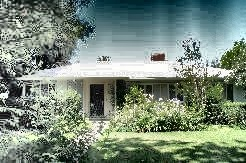
\includegraphics[width=0.45\textwidth]{./Figures/calhouse_230/0-resultado.jpg}
    }
%        \caption{Imagen Original. $\mathscr{H_Y}=0.207231$, $SSIM_R=1$, $SSIM_G=1$, $SSIM_B=1$}
        \label{fig:calhouse2300}
    \end{subfigure}
    ~ %add desired spacing between images, e. g. ~, \quad, \qquad, \hfill etc. 
      %(or a blank line to force the subfigure onto a new line)
    \begin{subfigure}[DI=1]{
        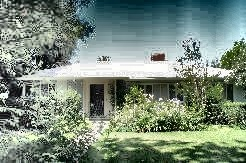
\includegraphics[width=0.45\textwidth]{./Figures/calhouse_230/1-resultado.jpg}   
    }
    %\begin{subfigure}[t]{0.45\textwidth}
%        \caption{Enhanced Image. $\mathscr{H_Y}=0.611275$, $SSIM_R=0.00897331$, $SSIM_G=0.00823064$, $SSIM_B=0.00851013$}
        \label{fig:calhouse2301}
    \end{subfigure}
    ~ %add desired spacing between images, e. g. ~, \quad, \qquad, \hfill etc. 
    %(or a blank line to force the subfigure onto a new line)
    \begin{subfigure}[ID=23]{
        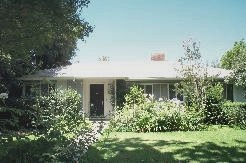
\includegraphics[width=0.45\textwidth]{./Figures/calhouse_230/23-resultado.jpg}
    }
    % \begin{subfigure}[t]{0.45\textwidth}
%        \caption{Enhanced Image.  $\mathscr{H_Y}=0.0350595$, $SSIM_R=0.416776$, $SSIM_G=0.403636$, $SSIM_B=0.417654$}
        \label{fig:calhouse23023}
    \end{subfigure} 
    \begin{subfigure}[ID=24]{
        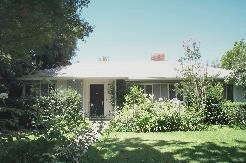
\includegraphics[width=0.45\textwidth]{./Figures/calhouse_230/24-resultado.jpg}
    }
    % \begin{subfigure}[t]{0.45\textwidth}
        %\caption{Enhanced Image using \cite{morepso}. $\mathscr{H_Y}=0.788927$, $SSIM_R=0.000204143$, $SSIM_G=0.0000526475$, $SSIM_B=0.0000518143$}
        \label{fig:calhouse23024}
    \end{subfigure}
    ~ %add desired spacing between images, e. g. ~, \quad, \qquad, \hfill etc. 
    %(or a blank line to force the subfigure onto a new line)
    \begin{subfigure}[ID=56]{
        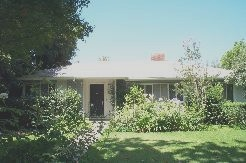
\includegraphics[width=0.45\textwidth]{./Figures/calhouse_230/56-resultado.jpg}
    }
    % \begin{subfigure}[t]{0.45\textwidth}
%        \caption{Enhanced Image.  $\mathscr{H_Y}=0.0350595$, $SSIM_R=0.416776$, $SSIM_G=0.403636$, $SSIM_B=0.417654$}
        \label{fig:calhouse23056}
    \end{subfigure} 
    \begin{subfigure}[Imagen Original]{
        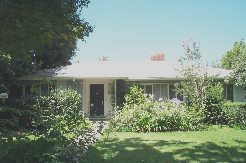
\includegraphics[width=0.45\textwidth]{./Figures/calhouse_230/calhouse_230.jpg}
    }
    % \begin{subfigure}[t]{0.45\textwidth}
        %\caption{Enhanced Image using \cite{morepso}. $\mathscr{H_Y}=0.788927$, $SSIM_R=0.000204143$, $SSIM_G=0.0000526475$, $SSIM_B=0.0000518143$}
        \label{fig:calhouse230orig}
    \end{subfigure}
    \caption{Imágenes visualmente relevantes obtenidas mediante $CMOPSO-CLAHE$. Las variables y decisión y métricas de las imágenes se muestran en la tabla \ref{tab:calhouse_230}.}\label{fig:anexocalhouse230}
\end{figure}


% \begin{table}[H]
% \centering
% \caption{Promedios de los tiempos de ejecución de algoritmo HE para las imágenes en escala de grises.}
% \label{tabla22}
% \begin{tabular}{|c|c|}
% \hline
% \begin{tabular}[c]{@{}c@{}}Nº de \\ ejecución\end{tabular} & \begin{tabular}[c]{@{}c@{}}t\\ (ms)\end{tabular} \\ \hline
% 1                                                          & 1,145                                            \\
% 2                                                          & 0,945                                            \\
% 3                                                          & 0,97                                             \\
% 4                                                          & 0,925                                            \\
% 5                                                          & 0,95                                             \\ \hline
% Promedio                                                   & \textbf{0.987}                                   \\ \hline
% \end{tabular}
% \end{table}


% En la Tabla \ref{tabla23} se muestran los promedios de los tiempos de ejecución del algoritmo MMCE para las imágenes en escala de grises.

% % Please add the following required packages to your document preamble:
% % \usepackage{multirow}
% \begin{table}[H]
% 	\centering
% 	\caption{Promedios de los tiempos de ejecución del algoritmo MMCE para las imágenes en escala de grises.}
% 	\label{tabla23}
% 	\begin{tabular}{|c|c|c|c|c|c|c|}
% 		\hline
% 		\multirow{2}{*}{Iter. (n)} & \multicolumn{5}{c|}{Nº de ejeciciones para el algoritmo MMCE} & \multirow{2}{*}{\begin{tabular}[c]{@{}c@{}}Promedios\\ t(ms)\end{tabular}} \\ \cline{2-6}
% 		& 1           & 2          & 3         & 4         & 5          &                                                                            \\ \hline
% 		1                          & 64,265      & 62,625     & 61,61     & 62,285    & 62,295     & \textbf{62,616}                                                            \\
% 		2                          & 165,805     & 171,24     & 169,655   & 170,515   & 170,295    & \textbf{169,502}                                                           \\
% 		3                          & 327,975     & 334,19     & 334,75    & 332,045   & 333,275    & \textbf{332,447}                                                           \\
% 		4                          & 564,035     & 574,15     & 571,185   & 573,45    & 568,735    & \textbf{570,311}                                                           \\
% 		5                          & 975,845     & 972,035    & 979,205   & 968,975   & 986,805    & \textbf{976,573}                                                           \\
% 		6                          & 1454,415    & 1471,145   & 1449,78   & 1452,97   & 1463,74    & \textbf{1458,41}                                                           \\
% 		7                          & 2037,11     & 2032,775   & 2041,54   & 2029,07   & 2038,735   & \textbf{2035,846}                                                          \\ \hline
% 	\end{tabular}
% \end{table}


% En la Tabla \ref{tabla24} se muestran los promedios de los tiempos de ejecución del algoritmo propuesto para las imágenes en escala de grises.

% % Please add the following required packages to your document preamble:
% % \usepackage{multirow}
% \begin{table}[H]
% 	\centering
% 	\caption{Promedios de los tiempos de ejecución del algoritmo propuesto para las imágenes en escala de grises.}
% 	\label{tabla24}
% 	\begin{tabular}{|c|c|c|c|c|c|c|}
% 		\hline
% 		\multirow{2}{*}{Iter. (n)} & \multicolumn{5}{c|}{Nº de ejeciciones para el algoritmo propuesto} & \multirow{2}{*}{\begin{tabular}[c]{@{}c@{}}Promedios \\ t(ms)\end{tabular}} \\ \cline{2-6}
% 		& 1            & 2           & 3           & 4          & 5          &                                                                             \\ \hline
% 		1                          & 62,105       & 63,055      & 61,99       & 62,445     & 62,955     & 62,51                                                                       \\
% 		2                          & 166,74       & 169,645     & 168,34      & 168,435    & 169,34     & 168,5                                                                       \\
% 		3                          & 327,175      & 332,58      & 331,765     & 332,755    & 331,52     & 331,159                                                                     \\
% 		4                          & 565,245      & 576,84      & 574,47      & 573,6      & 572,15     & 572,461                                                                     \\
% 		5                          & 976,57       & 973,22      & 968,35      & 970,245    & 975,26     & 972,729                                                                     \\
% 		6                          & 1463,175     & 1474,82     & 1458,765    & 1459,83    & 1470,06    & 1465,33                                                                     \\
% 		7                          & 2047,435     & 2040,82     & 2041,915    & 2039,95    & 2044,16    & 2042,856                                                                    \\ \hline
% 	\end{tabular}
% \end{table}

